% bei Standalone in documentclass noch:
% \RequirePackage{luatex85}

\documentclass[captions=tableheading, titlepage= firstiscover, parskip = half , bibliography=totoc]{scrartcl}
%paper = a5 für andere optinen
% titlepage= firstiscover
% bibliography=totoc für bibdateien
% parskip=half  Veränderung um Absätze zu verbessern

\usepackage{scrhack} % nach \documentclass
\usepackage[aux]{rerunfilecheck}
\usepackage{polyglossia}
\usepackage[style=numeric, backend=biber]{biblatex} % mit [style = alphabetic oder numeric] nach polyglossia
\addbibresource{lit.bib}
\setmainlanguage{german}

\usepackage[autostyle]{csquotes}
\usepackage{amsmath} % unverzichtbare Mathe-Befehle
\usepackage{amssymb} % viele Mathe-Symbole
\usepackage{mathtools} % Erweiterungen für amsmath
\usepackage{fontspec} % nach amssymb
% muss ins document: \usefonttheme{professionalfonts} % für Beamer Präsentationen
\usepackage{longtable}

\usepackage[
math-style=ISO,    % \
bold-style=ISO,    % |
sans-style=italic, % | ISO-Standard folgen
nabla=upright,     % |
partial=upright,   % /
]{unicode-math} % "Does exactly what it says on the tin."
\setmathfont{Latin Modern Math}
% \setmathfont{Tex Gyre Pagella Math} % alternativ

\usepackage[
% die folgenden 3 nur einschalten bei documenten
locale=DE,
separate-uncertainty=true, % Immer Fehler mit ±
per-mode=symbol-or-fraction, % m/s im Text, sonst \frac
]{siunitx}

% alternativ:
% per-mode=reciprocal, % m s^{-1}
% output-decimal-marker=., % . statt , für Dezimalzahlen

\usepackage[
version=4,
math-greek=default,
text-greek=default,
]{mhchem}

\usepackage[section, below]{placeins}
\usepackage{caption} % Captions schöner machen
\usepackage{graphicx}
\usepackage{grffile}
\usepackage{subcaption}

% \usepackage{showframe} Wenn man die Ramen sehen will

\usepackage{float}
\floatplacement{figure}{htbp}
\floatplacement{table}{htbp}

\usepackage{mhchem} %chemische Symbole Beispiel: \ce{^{227}_{90}Th+}


\usepackage{booktabs}

 \usepackage{microtype}
 \usepackage{xfrac}

 \usepackage{expl3}
 \usepackage{xparse}

 % \ExplSyntaxOn
 % \NewDocumentComman \I {}  %Befehl\I definieren, keine Argumente
 % {
 %    \symup{i}              %Ergebnis von \I
 % }
 % \ExplSyntaxOff

 \usepackage{pdflscape}
 \usepackage{mleftright}

 % Mit dem mathtools-Befehl \DeclarePairedDelimiter können Befehle erzeugen werden,
 % die Symbole um Ausdrücke setzen.
 % \DeclarePairedDelimiter{\abs}{\lvert}{\rvert}
 % \DeclarePairedDelimiter{\norm}{\lVert}{\rVert}
 % in Mathe:
 %\abs{x} \abs*{\frac{1}{x}}
 %\norm{\symbf{y}}

 % Für Physik IV und Quantenmechanik
 \DeclarePairedDelimiter{\bra}{\langle}{\rvert}
 \DeclarePairedDelimiter{\ket}{\lvert}{\rangle}
 % <name> <#arguments> <left> <right> <body>
 \DeclarePairedDelimiterX{\braket}[2]{\langle}{\rangle}{
 #1 \delimsize| #2
 }

\setlength{\delimitershortfall}{-1sp}

 \usepackage{tikz}
 \usepackage{tikz-feynman}

 \usepackage{csvsimple}
 % Tabellen mit \csvautobooktabular{"file"}
 % muss in table umgebung gesetzt werden


% \multicolumn{#Spalten}{Ausrichtung}{Inhalt}

\usepackage{hyperref}
\usepackage{bookmark}
\usepackage[shortcuts]{extdash} %nach hyperref, bookmark

\newcommand{\ua}[1]{_\symup{#1}}
\newcommand{\su}[1]{\symup{#1}}


\title{Versuch 702}
\subtitle{Aktivierung mit Neutronen}
\author{Jonah Nitschke\\
        lejonah@web.de \and
        Sebastian Pape\\
        sepa@gmx.de}
\date{Durchführung: 18.04.2017\\
      Abgabe: 25.04.2017}



\begin{document}

\maketitle

\section{Theorie}

\subsection{Zielsetzung}

Der Versuch 702 setzt sich mit dem radioaktiven Zerfall von Aktivierten Atomkernen auseinander.
Das Ziel des Versuches ist es die Halbwertszeit des Isotopes $\ce{^{116}_{49}In}$
und eines Rhodiumisomeres zu bestimmen.

\subsection{Theoretische Grundlagen}

Damit instabile Kerne erzeugt werden, werden stabile Kene mit Neutronen beschossen.
Der Vorteil der Neutronenaktivierung liegt darin, dass die ladungsneutralen
Neutronen weniger Energie benötigen, um die Kerne zu aktivieren, da sie
nicht die Coulomb-Barriere des geladenen Kernes überwinden müssen.

Eine Allgemeine Kernreaktion eines Beispielkernes $\ce{^{m}_{z}A}$ sieht
folgendermaßen aus:

\begin{equation*}
  \ce{^{m}_{z}A + ^{1}_{0}n -> ^{m+1}_{z}A^{*} -> ^{m+1}_{z}A + \gamma} .
\end{equation*}

$\ce{^{m}_{z}A^{*}}$ ist dabei der sogenannte Zwischenkern oder auch Compoundkern.
Seine Energie ist im Vergleich zu dem Ausgangskern um die kinetische Energie
des Neutrons und der Bindungsenergie höher.
Bei geringer kinetischer Energie des Neutrons ist die eingebrachte Energie
zu gering um ein Nukleon oder ein Neutron wieder abzugeben. Deshalb wird
nach etwa $\SI{e-16}{\second}$ ein $\gamma$-Quant abgegeben, sodass der Kern
wieder in seinen Grundzustand zurückfällt. Dieser Kern ist immernoch instabil,
hat aber eine deutlich längere Lebensdauer als der Zwischenkern.
Die Zerfallsreihe dieses Kerns läuft wie folgt ab:

\begin{equation*}
  \ce{^{m+1}_{z}A -> ^{m+1}_{z+1}C + \beta^{-} + E_{kin} + \bar{\nu}_{e}}.
\end{equation*}

Dieser Zerfall ist ein erlaubter Zerfall, da die Masse der linken Seite
größer ist als die Gesamtmasse der rechten Seite. Der Massenunterschied
ist durch die Einsteinsche Energie-Masse Beziehung einzusehen.

\begin{equation}
  \label{eqn:Einstein}
  \Delta E = \Delta mc^2
\end{equation}

Die Masse wird in Form von kinetischer Energie an das $\beta^{-}$- und
$\bar{\nu}_{e}$-Teilchen abgegeben ($\bar{\nu}_{e}$ ist ein Antineutrino).

Wenn Neutronen auf stabile Atomkerne geschossen werden, ist die
charakteristische Größe, dass ein Neutron von einem Atomkern eingefangen wird
der Wirkungsquerschnitt. Er ist über die Formel

\begin{equation}
  \label{eqn:Wirkungsquerschnitt}
  \sigma = \frac{u}{nKd}
\end{equation}

definiert, wenn Neutronen auf eine Folie mit einem Flächeninhalt von
$\SI{1}{\centi\meter^2}$ geschossen werden.
Dabei ist $n$ die Anzahl der abgeschossenen Neutronen, $u$ die
Anzahl der eingefangenen Neutronen, $d$ die Dicke der beschossenen Fläche und
$K$ die Anzahl der Atome pro Quadratcentimeter in der Folie.
Der Wirkungsquerschnitt wird in der Einheit $\SI{e-24}{\centi\meter^2} = \SI{1}{\barn}$
gemessen.
Bei den abgeschossenen Neutronen wird zwischen schnellen und langsamen Neutronen
unterschieden. Die beiden unterscheiden sich, wie der Name es suggeriert
lediglich in ihrer Geschwindigkeit $v$. Als Kriterium dieser Klassifizierung
dient die De-Broglie-Wellenlänge $\lambda$, die definiert ist über:

\begin{equation}
  \label{eqn:debroglie}
  \lambda = h / m_n v.
\end{equation}

Ist $\lambda$ groß gegenüber dem Kernradius $R (\approx \SI{e-14}{\meter})$
handelt es sich um schnelle Neutronen. Andersherum handelt es sich um langsame
Neutronen. Bei langsamen Neutronen ist der Wirkungsquerschnitt deutlich größer
als bei schnellen Neutronen, weshalb sich langsame Neutronen besser für die Aktivierung
von Atomkernen eignen. Es stellt sich heraus, dass $\sigma$ reziprok
von der Geschwindigkeit $v$ der Neutronen abhängt.

Bei der Aktivierung der Proben müssen langsame Neutronen zunächst erzeugt werden.
Schnelle Neutronen lassen sich aus verschieden Reaktionen gewinnen. Der
Abbremsungsvorgang wird über elastische Stöße realisiert.
Dabei stoßen die Neutronen mit den Kohlenwasserstoffen in einem Paraffinmantel,
der um die Neutronenquelle anliegt. Zum Abbremsen der schnellen Neutronen
eignen sich ähnlich schwere Moleküle besser, da aus den Formeln des elastischen
Stoßes hervorgeht, dass der größte Energieübertrag zweier elastisch stoßender
Teilchen  bei gleicher Masse erfolgt. Deshalb eignet sich Parrafin, weil der in
dem Paraffin enthaltene Wasserstoff beinahe die selbe Masse wie ein
Neutron besitzt. Sind die Neutronen auf eine Geschwindigkeit von
$\SI{2,2}{\kilo\meter\per\second}$ abgebremst, werden sie auch als
thermische Neutronen bezeichnet.

Der radioaktive Zerfall von instabilen Atomkernen lässt sich durch ein
Exponentialgesetzt beschreiben. Die Anzahl der zur Zeit $t$ noch nicht
Zerfallenen Kerne lässt sich wie folgt berechnen.

\begin{equation}
  \label{eqn:expo}
  N(t) = N_0\exp^{-\lambda t}
\end{equation}

Dabei ist $N_0$ die anfängliche Anzahl der instabilen Kerne und $\lambda$
die Zerfallskonstante.

Die Zerfallsreihen der verwendeten Proben Indium und Rhodium sind im Folgenden
dargestellt.

\begin{align}
  \label{eqn:Indium}
  \ce{^{115}_{49}In + ^{1}_{0}n &-> ^{116}_{49}In -> ^{116}_{50}Sn + \beta^- + \bar{\nu}_e} \\
  \label{eqn:Rhodium}
  \ce{^{103}_{45}Rh + ^{1}_{0}n}&
  \begin{cases}
  \overset{10\%}{\ce{->}} \ce{^{104i}_{45}Rh
  -> ^{104}_{45}Rh} + \gamma \ce{-> ^{104}_{46}Pd + \beta^{-} + \bar{\nu}_e} \\
  \overset{90\%}{\ce{->}} \ce{^{104}_{45}Rh -> ^{104}_{46}Pd + \beta^{-} + \bar{\nu}_e}
  \end{cases}.
\end{align}

\section{Durchführung}

Die zu untersuchenden Proben wurden im Vorhinein aktiviert. Für die Aktivierung
wird die Apparatur aus Abb. \ref{fig:Aktivierung} verwendet.

\begin{figure}
  \centering
  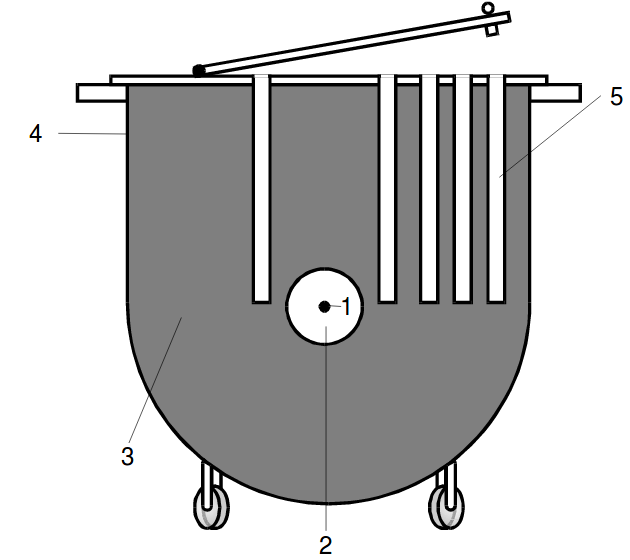
\includegraphics[width=7.50cm, height=6cm]{V702_Aktivierung.png}
  \caption{Schematische Darstellung der Aktivierungsvorrichtung\cite{anleitung01}}
  \label{fig:Aktivierung}
\end{figure}

Die in Abb. \ref{fig:Aktivierung} aufgeführten Makierungen sind wie folgt erklärt.

\begin{description}
  \item[1] Quelle schneller Neutronen
  \item[2] Bleiabschirmung
  \item[3] Paraffin
  \item[4] Stahlbehälter
  \item[5] Aktivierungsbohrungen
\end{description}

Vor der ersten Messung muss der Nullwert bestimmt werden. Dafür wird eine
Messung über $\SI{900}{\second}$ ohne Probe gemacht.
Danach wurden die zu untersuchenden Proben in den Aufbau eingelegt.
Es wurden das Isotop Indium-116 ($\ce{^{116}In}$)
und ein Rhodiumisomer ($\ce{^{104}Rh}$ \& $\ce{^{104i}Rh}$) untersucht.
Für das Indiumisotop ist eine Messzeit von einer Stunde mit einem Messintervall von
$\Delta t = \SI{240}{\second}$ gewählt worden. Für das Rhodiumisomer ist eine
Messzeit von $\SI{12}{\minute}$ angesetzt worden, mit einem Messintervall
$\Delta t$ von $\SI{15}{\second}$.

Die Messungen sind mit dem Aufbau, der in Abb. \ref{fig:Aufbau} dargestellt ist,
zu realisieren. Der Aufbau besteht grundlegend aus einem Geiger-Müller-Zählrohr,
einen Impulsverstärker und einem Zählwerk mit zwei Displays.
Das Geiger-Müller-Zählrohr misst die radioaktiven Zerfälle in Form
eines eletrischen Impulses. Dieser wird durch einen Impulsverstärker geschickt und
letztendlich von einem Zählwerk registriert. Das Zählwerk besitzt zwei Displays,
sodass kontinuierlich gemessen werden kann.

\begin{figure}
  \centering
  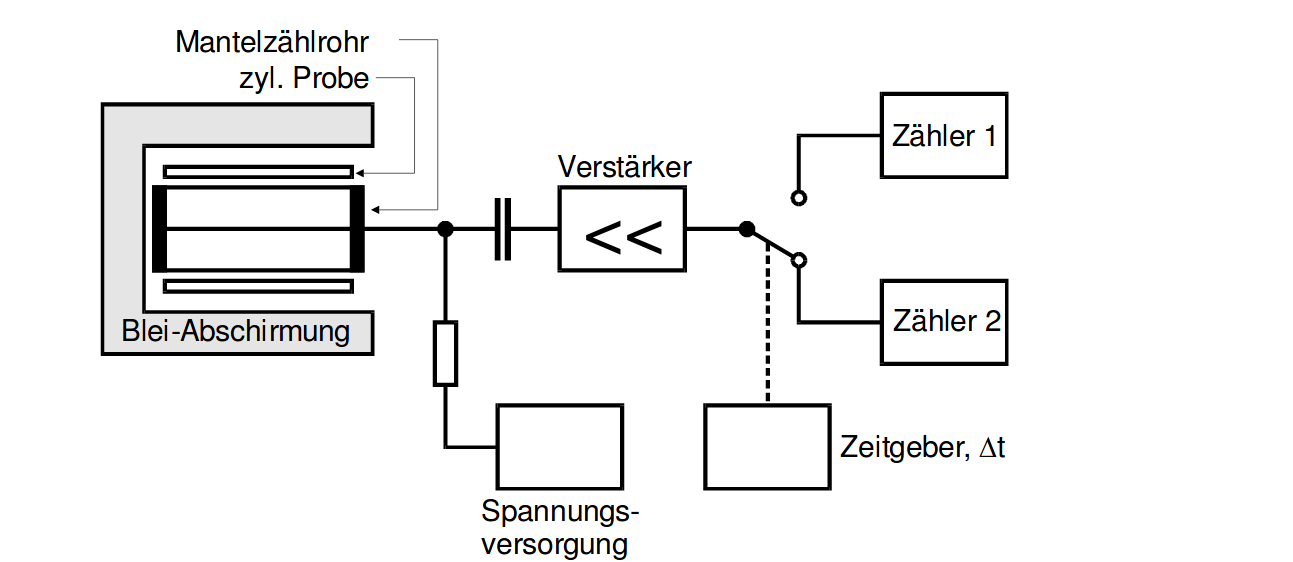
\includegraphics[width=\textwidth]{V702_Aufbau.png}
  \caption{Schematischer Versuchsaufbau\cite{anleitung01}}
  \label{fig:Aufbau}
\end{figure}

Die Probe wird zu Beginn der Messung gemäß Abb. \ref{fig:Aufbau} eingelegt.
Vor dem Einlegen der Probe muss das Messintervall $\Delta t$ an dem Zählwerk
eingestellt werden. Die Messwerte können an dem Zählwerk erhoben werden.

\newpage

\printbibliography

\end{document}
